bron Ug= 1mhz, 20vpp

In de afbeeldingen is channel 1 nabij en channel 2 verre eind

\subsection{Capacitieve overspraak}
\begin{enumerate}
    \item Meet de capacitieve overspraak aan zowel het nabije eind (XN) als het verre eind (XV).
    Vergelijk de twee spanningen zowel in amplitude als in fase. Wat valt op bij het vergelijken
    van deze spanningen. Verklaar en onderbouw de bevindingen met de bijbehorende theorie.

    \begin{figure}[H]
        \centering
        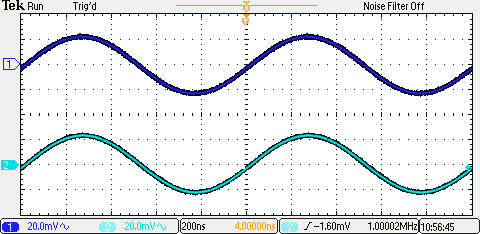
\includegraphics[scale=0.5]{Capacitieve overspraak probe.PNG}
        \caption{capacitief met probe}
        \label{fig:capacitief met probe}
    \end{figure}

    \begin{figure}[H]
        \centering
        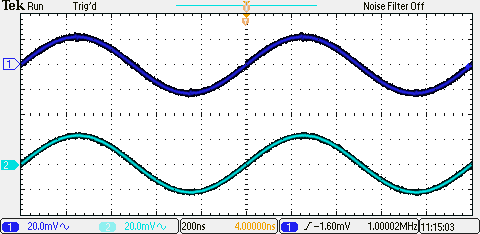
\includegraphics[scale=0.5]{Capacitieve overspraak coax.PNG}
        \caption{capacitief met coax}
        \label{fig:capacitief met coax}
    \end{figure}

    Bij de Capacitieve overspraak is te zien in afbeelding \ref{fig:capacitief met probe} en \ref{fig:capacitief met coax} dat er nagenoeg geen verschil zit tussen het begin en het eind. Dit komt omdat de lijn aan het eind niet is afgesloten en hierdoor het signaal in fase terug komt.


    \item  Bereken met behulp van de meetresultaten en de theorie uit ref. 3. de waarde van de koppel- capaciteit tussen de twee geleiders.
    
    \begin{equation}
        \begin{split}
            U_{onc} = U_{ovc} &= Z_{0} \cdot \frac{j \omega c_{12} \cdot u_{g}}{2}\\
            0,04 &= 220 \cdot \frac{10^6 c_{12} \cdot 20}{2}\\
            &\Downarrow \\
            C_{12} &= 181 nF
        \end{split}
    \end{equation}

    \item Evalueer het resultaat. Klopt de ordegrootte van het resultaat en op basis waarvan is dit beoordeeld.
\end{enumerate}

\newpage

\subsection{Inductieve overspraak}
\begin{enumerate}
    \item Meet de inductieve overspraak aan zowel het nabije eind (XN) als het verre eind (XV). Vergelijk de twee spanningen zowel in amplitude als in fase. Wat valt op bij het vergelijken
    van deze spanningen. Verklaar en onderbouw de bevindingen met de bijbehorende theorie.

    \begin{figure}[H]
        \centering
        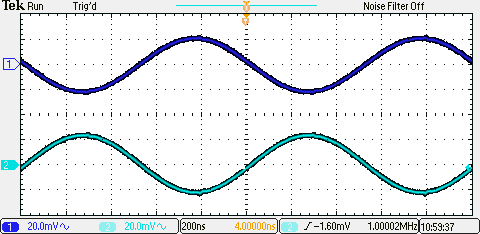
\includegraphics[scale=0.5]{Inductieve overspraak probe.PNG}
        \caption{Inductief met probe}
        \label{fig:Inductief met probe}
    \end{figure}

    \begin{figure}[H]
        \centering
        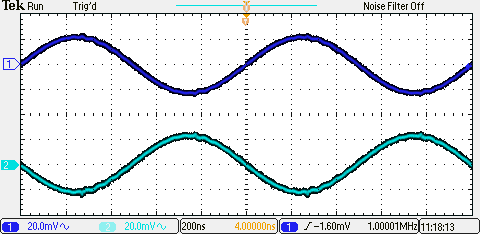
\includegraphics[scale=0.5]{Inductieve overspraak coax.PNG}
        \caption{Inductief met coax}
        \label{fig:Inductief met coax}
    \end{figure}

    Bij de Inductieve overspraak is te zien in afbeelding \ref{fig:Inductief met probe} en \ref{fig:Inductief met coax} dat er bij XN het signaal gemeten word met een 180 graden fase verschuiving. Dit komt omdat de lijn aan het eind is kortgesloten en hierdoor het signaal in fase gedraaid terug komt.
    
    \item Bereken met behulp van de meetresultaten en de theorie uit ref. 3 de waarde van de
    mutuele zelfinductie tussen de twee geleiders.

    \begin{equation}
        \begin{split}
            U_{oni} &= j \omega L_{M} \cdot \frac{U_{g}}{2 \cdot Z_{0}}\\
            0,04 &= 10^6 L_{M} \cdot \frac{20}{2 \cdot 220}\\
            &\Downarrow \\
            L_{M} &= 8,8 \mu H
        \end{split}
    \end{equation}

    \item Evalueer het resultaat. Klopt de ordegrootte van het resultaat en op basis waarvan is dit
    beoordeeld.

\end{enumerate}

\newpage

\subsection{Gelijktijdig capacitieve- en inductieve overspraak}
\begin{enumerate}
    \item Sluit de storende geleider (1) af met de karakteristieke impedantie van de lijn en leg uit
    waarom de overspraak op geleider 2 zowel een capacitief als een inductief deel heeft.

    \begin{figure}[H]
        \centering
        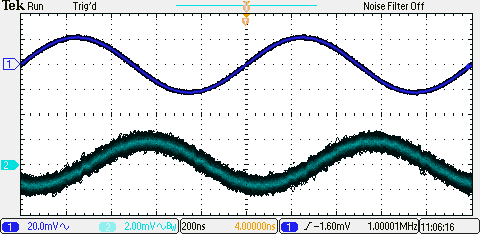
\includegraphics[scale=0.5]{Gelijktijdige overspraak probe.PNG}
        \caption{Gelijktijdig met probe}
        \label{fig:Gelijktijdig met probe}
    \end{figure}

    \begin{figure}[H]
        \centering
        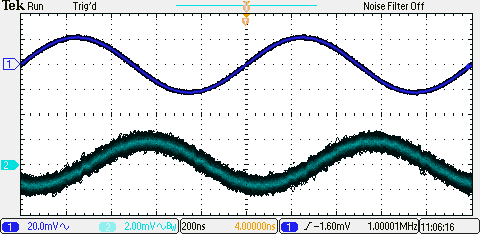
\includegraphics[scale=0.5]{Gelijktijdige overspraak probe.PNG}
        \caption{Gelijktijdig met coax}
        \label{fig:Gelijktijdig met coax}
    \end{figure}

    Bij de Gelijktijdige overspraak is te zien in afbeelding \ref{fig:Gelijktijdig met probe} en \ref{fig:Gelijktijdig met coax} dat er bij XN het signaal gemeten word met een fase verschuiving en dat bij XV ook een fase verschuiving gemeten wordt waarbij er ook verschil zit in amplitude waarbij het signaal bij XN ongeveer 10x zo groot is als bij XV. Dit komt doordat ....

    \item Meet de overspraak spanning op de slachtoffergeleider (2) aan zowel de nabije zijde (XN) als de verre zijde (XV).

    \item Verklaar aan de hand van de theorie waarom deze spanningen er zo uit zien.
    
    \item Verklaar de amplitude van de overspraak aan de nabije zijde doormiddel van een berekening.
    
    \begin{equation}
        \begin{split}
            U_{onc} &= Z_{0} \cdot \frac{j \omega C \cdot \frac{Z_{0}}{Z_{0}+ Z_{0}} \cdot U_{g}}{2}\\
            U_{onc} &= 220 \cdot \frac{10^6 \cdot 1,8 \cdot 10^{-11} \cdot 0,5 \cdot 20}{2}\\
            &\Downarrow \\
            U_{onc} &= 0,0198 V
            \\
            \\
            \\
            U_{oni} &= j \omega L_{M} \cdot \frac{U_{g}}{4 \cdot Z_{0}}\\
            U_{oni} &= 10^6 \cdot 8,8 \cdot 10^{-7} \cdot \frac{20}{2 \cdot 220}\\
            &\Downarrow \\
            U_{oni} &= 0,02 V\\
            \\
            \\
            \\
            U_{on} &= U_{onc} + U_{oni}\\
            &\Downarrow \\
            U_{on} &= 0,0398 V
        \end{split}
    \end{equation}

\end{enumerate}
